\subsection{Flapping and Bending of a Monofin}
An archetype of fluid-structure interaction is the flapping of a flag pole in a steady wing and the mutual interaction of the pole with its surrounding fluid. This phenomenon is also of interest in various other engineering applications such as locomotion using a monofin \cite{luersen2006computationally}, sails and understanding the flapping of flexible structures, and possible application of energy harvesting \cite{allen2001energy} and turbulence reduction \cite{shen2003turbulent}. Here we focus on calculating the sensitivity of structure response to the change in its shape since the application of the immersed boundary method for such problems has already been demonstrated in the work of Kim et al. \cite{kim2007penalty}. The physical domain for this problem is shown in Figure \ref{fig:C5_flagPolePhysical}. The boundary conditions are selected as constant velocity at inlet, free slip boundary conditions on top and bottom walls, and outflow boundary condition at the outlet.
%
\begin{figure}[H]
    \centering
    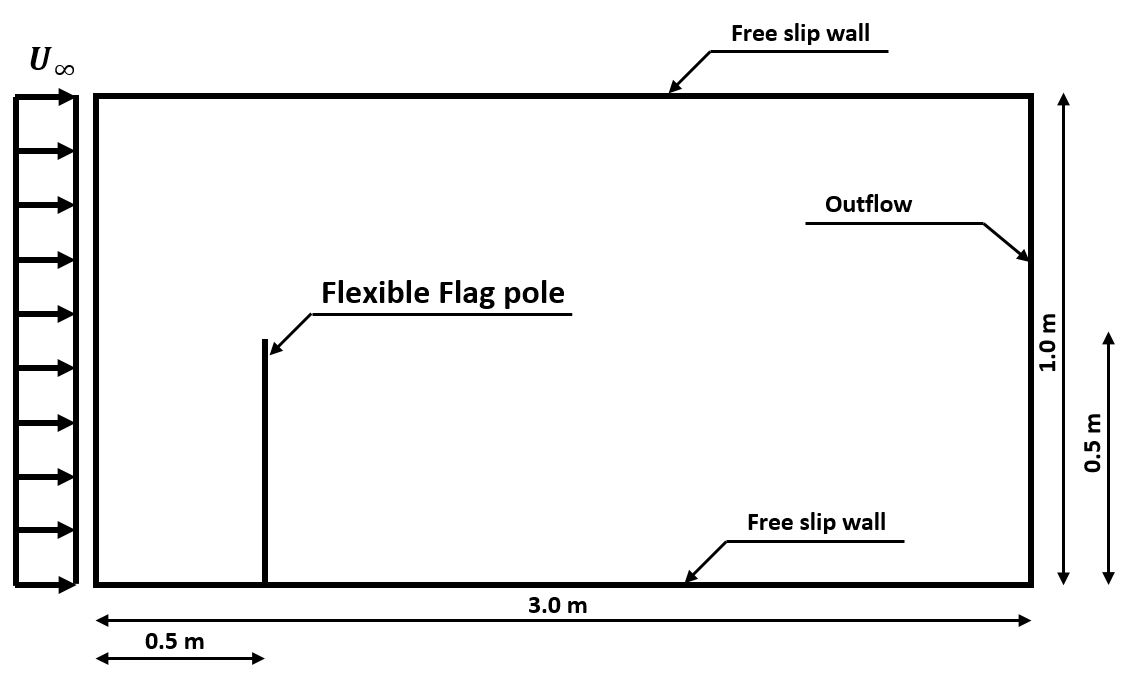
\includegraphics[width=9.00cm]{Chapter_5/figure/flagPole_domain_shape.jpg}
    \caption{Physical domain for the bending monofin.}
    \label{fig:C5_flagPolePhysical}
\end{figure}
%
As the cross-flow starts, the monofin will start vibrating due to aerodynamic loads. Due to the sudden start of the flow, the loading on the structure mimics the same characteristic as step function loading. Hence, we expect the structural response to have similar characteristics. This will provide us with more insight into the dynamic response of the system. 

The monofin structure is modeled using Euler-Bernoulli beam theory with three degrees of freedom at each node. The monofin is made of Aluminium with $E = 68.9$ GPa, and $\rho = 2.7 \times 10^3 \text{ Kg/m}^3$. The cross-section is defined as a circle with the diameter of $4 mm$. Due to the unsteady nature of the problem, the Newmark-beta method is used for explicit time integration of the structural equation of motion. As in previous problems, the pressure load is transferred to the structure using regularized delta function and the effect of location and velocity of the Lagrangian nodes of the structure are reflected through the IB forcing term of Equation \eqref{eq:C3_virtualBoundaryMethod}. For this problem, we considered at the unsteady response of two different cases of the monofin, each at a different length. The Reynolds number for this problem is fixed at $100$ to make sure that the Laminar flow assumption is met for the simulation. The time history of monofin tip displacement is shown in Figure \ref{fig:C5_timeHistoryTipDisplacement}. As we increase the length of the beam, the frequency of oscillation decreases. This is true since by increasing the length, the bending stiffness of the structure decreases, which results in a lower frequency of oscillation.
%
\begin{figure}[H]
    \centering
    \subfigure[$L = 0.5 \text{ m}$]
    {
    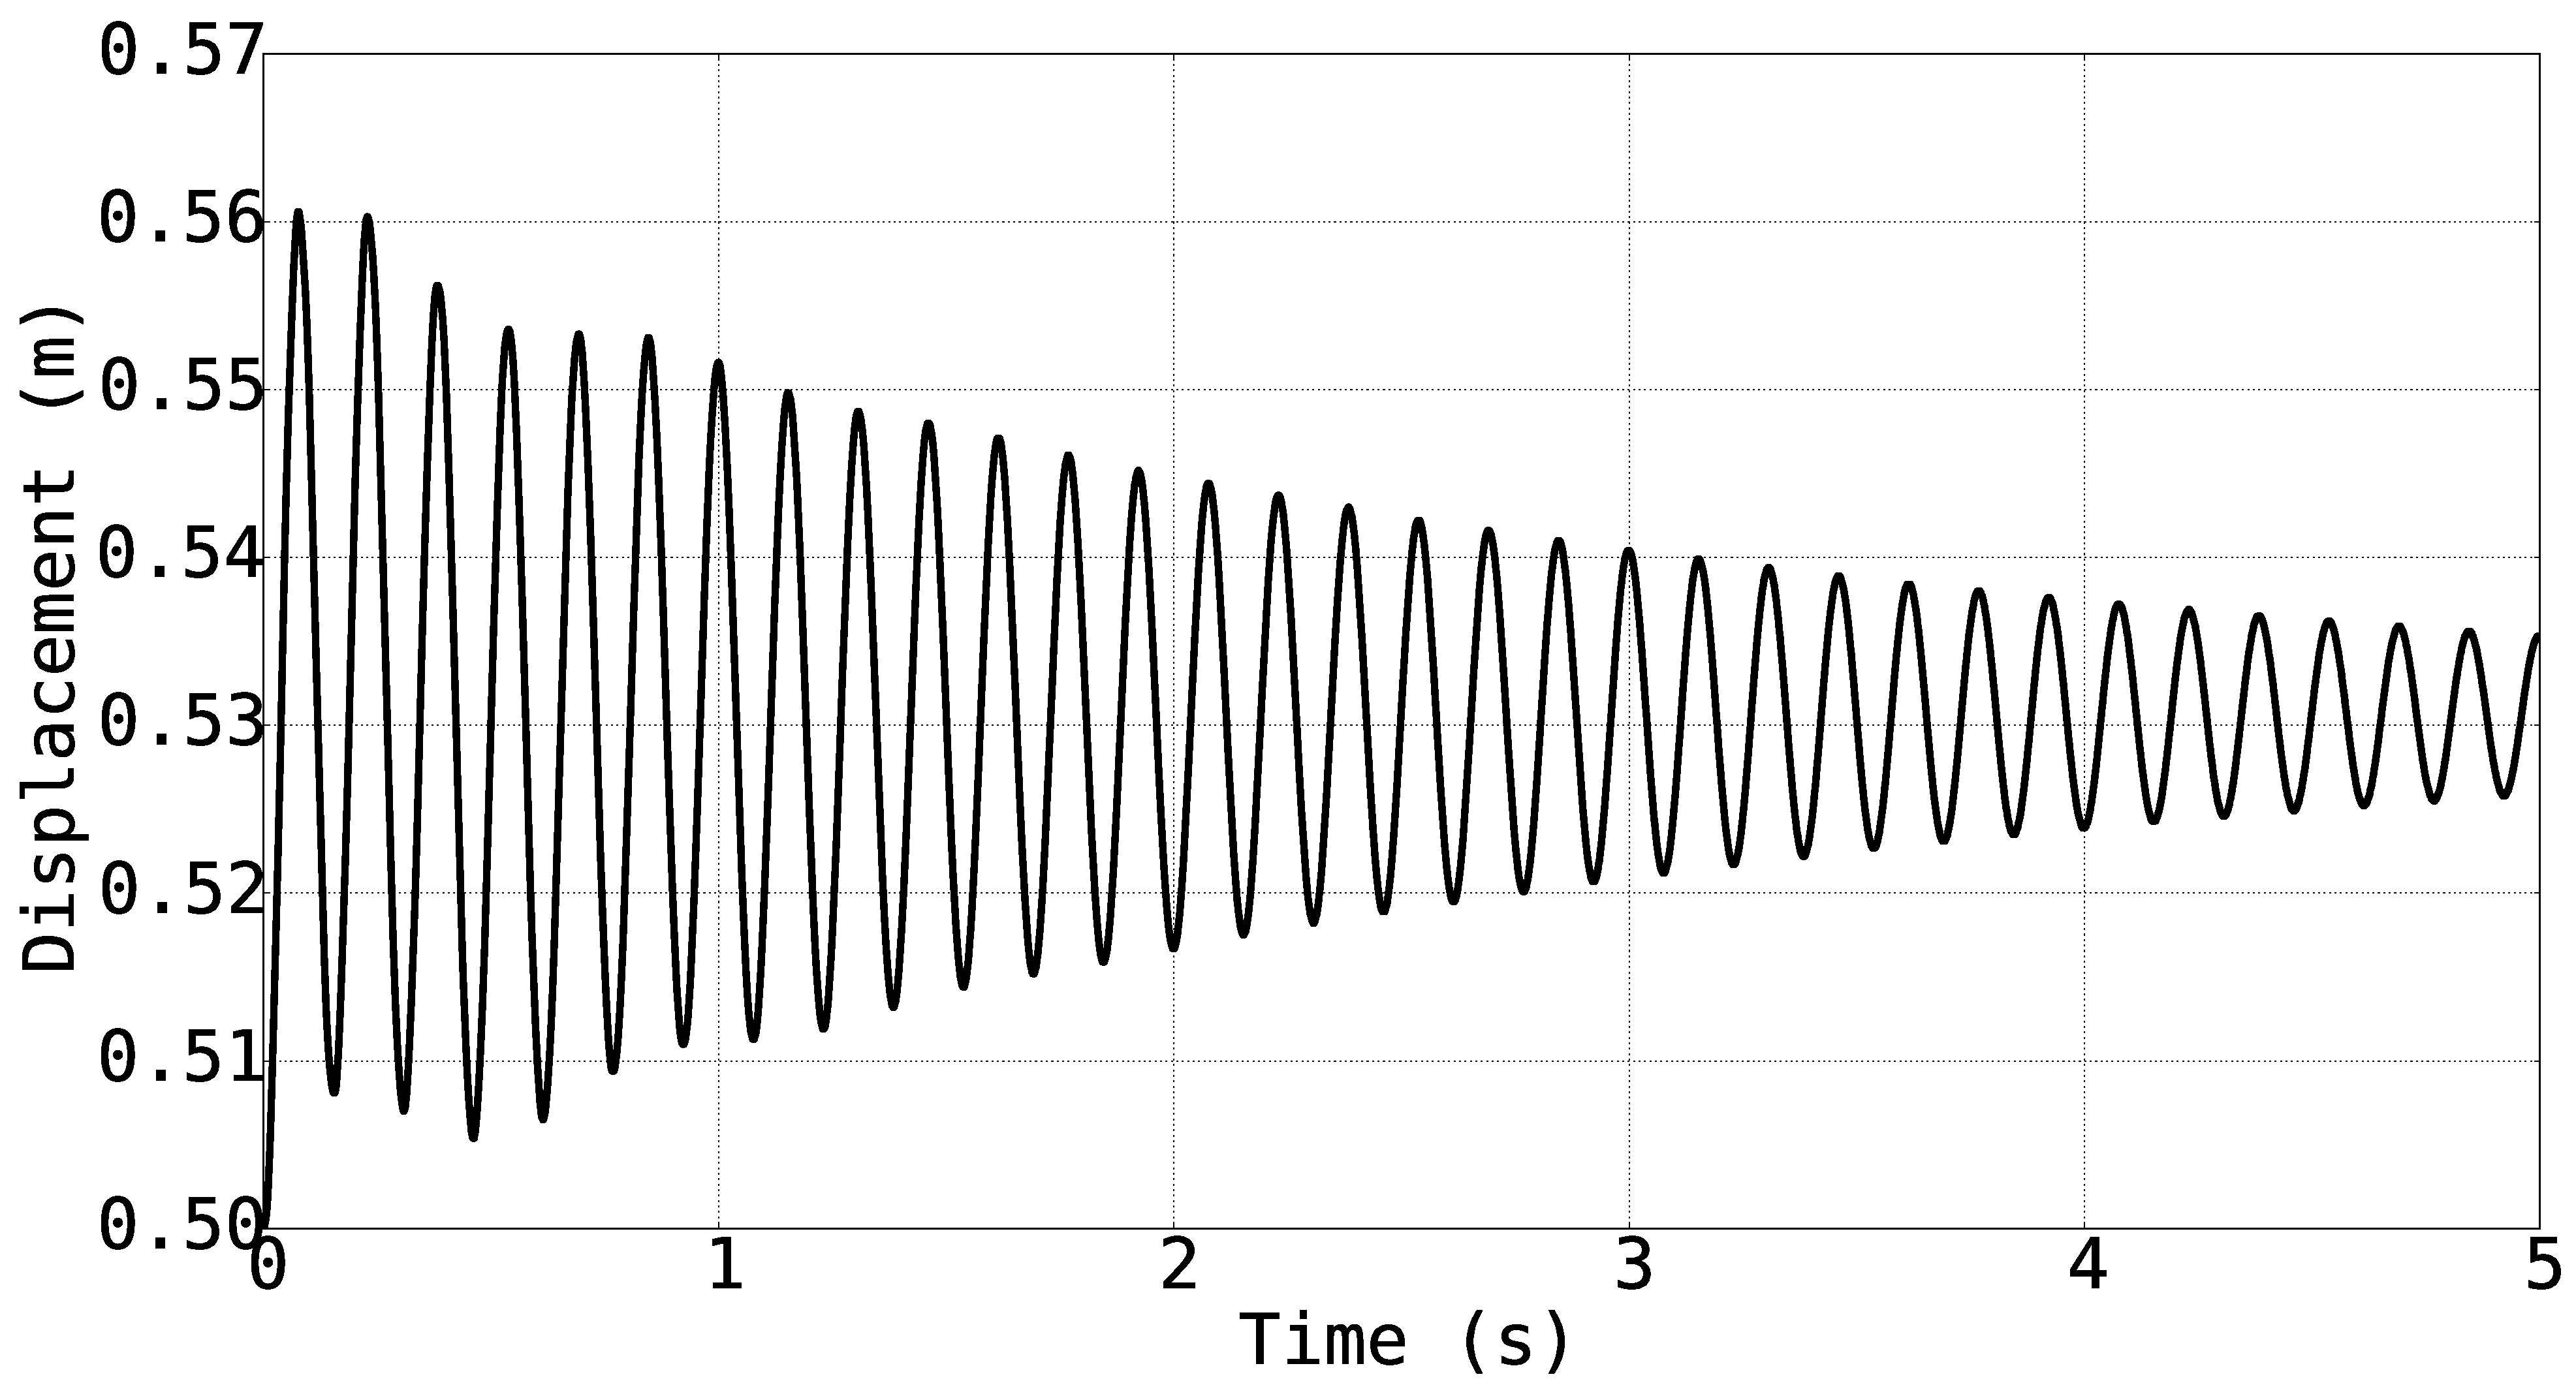
\includegraphics[width=6.5cm]{Chapter_5/figure/monofin_disp_L05.eps}
    \label{fig:C5_thinAirfoil}
    }
    \quad
    \subfigure[$L = 0.75 \text{ m}$]
    {
    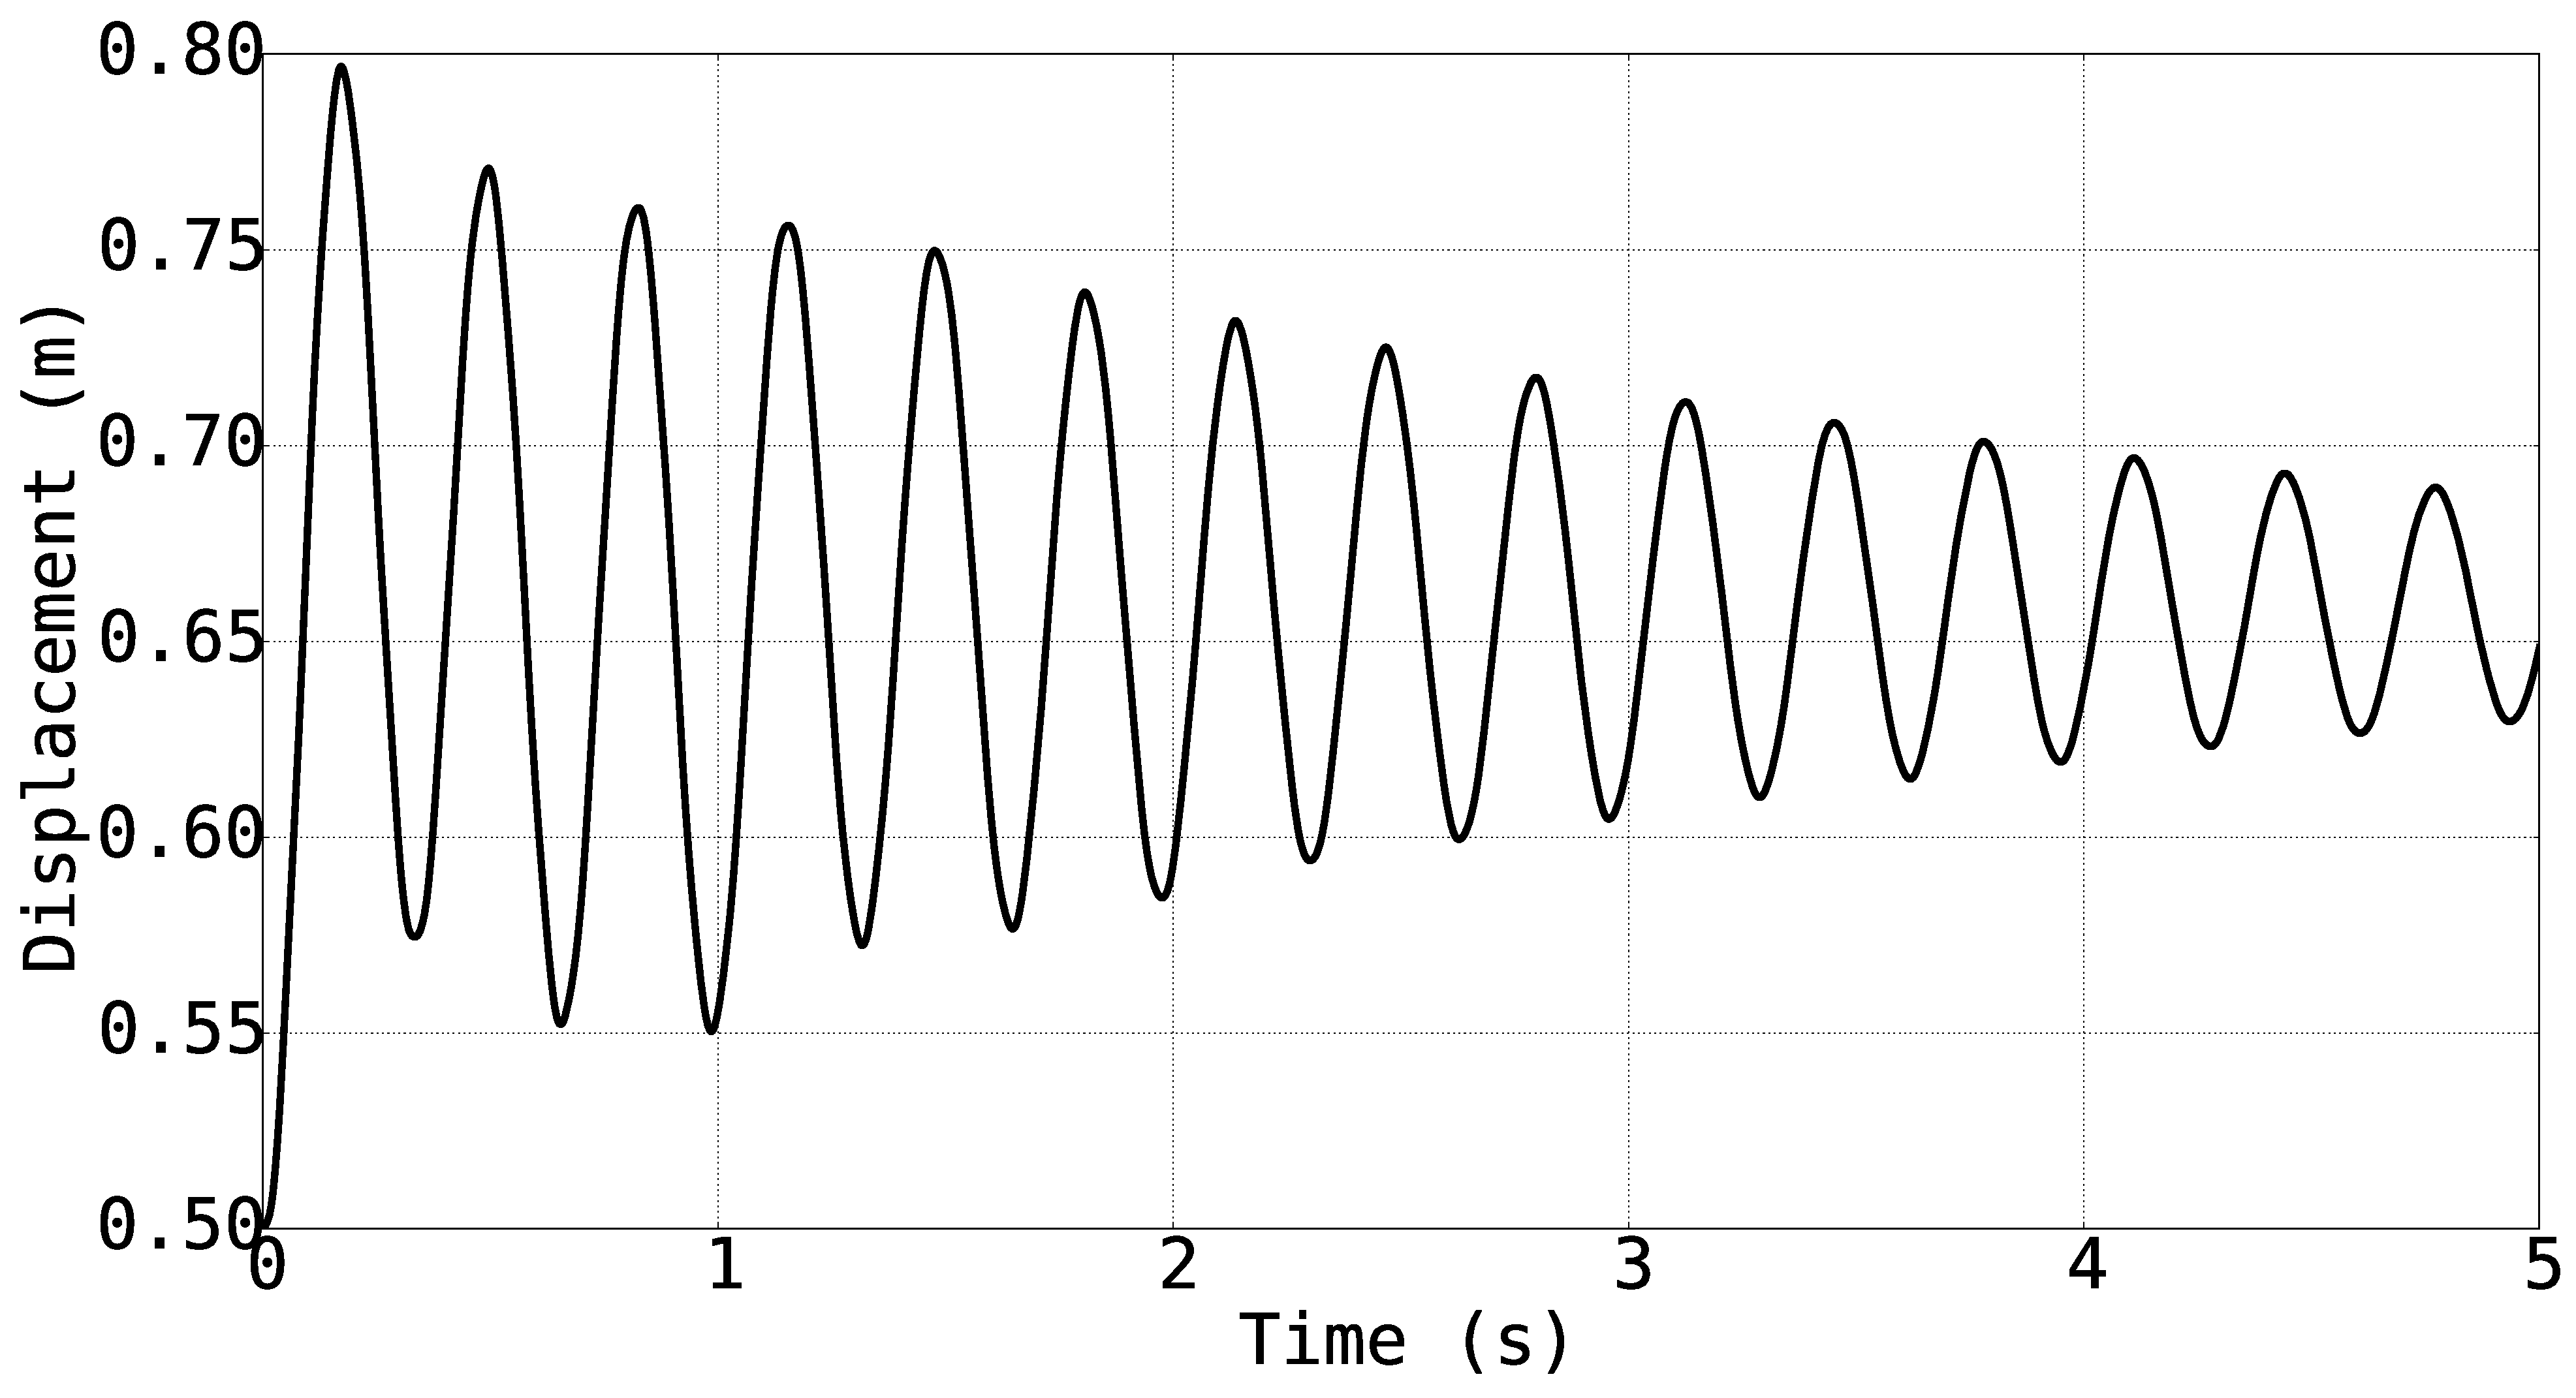
\includegraphics[width=6.5cm]{Chapter_5/figure/monofin_disp_L75.eps}
    \label{fig:C5_thickAirfoil}
    }
    \caption{Time history of the monofin tip displacement in cross-flow.}
    \label{fig:C5_timeHistoryTipDisplacement}
\end{figure}
%
Another important aspect of Figure \ref{fig:C5_timeHistoryTipDisplacement} is the viscous damping feature of the tip displacement movement. The structural model does not include viscous damping and the effect seen in Figure \ref{fig:C5_timeHistoryTipDisplacement} is purely due to the multidisciplinary interaction of fluid and structure for this problem. It is clear that the longer monofin experiences lower damping which is due to lower frequency and therefore, the lower velocity of the structure. This will result in less damping force since the viscous damping is proportional to the velocity of the structure. To better see the flow structure behind the monofin, time snapshots of the u-velocity and pressure contours are shown in Figure \ref{fig:C5_monofinTimeSnapShotVelocity} and \ref{fig:C5_monofinTimeSnapShotPressure} respectively.
%
\begin{figure}[H]
    \centering
    \subfigure[$t = 0.1 \text{ sec}$]
    {
    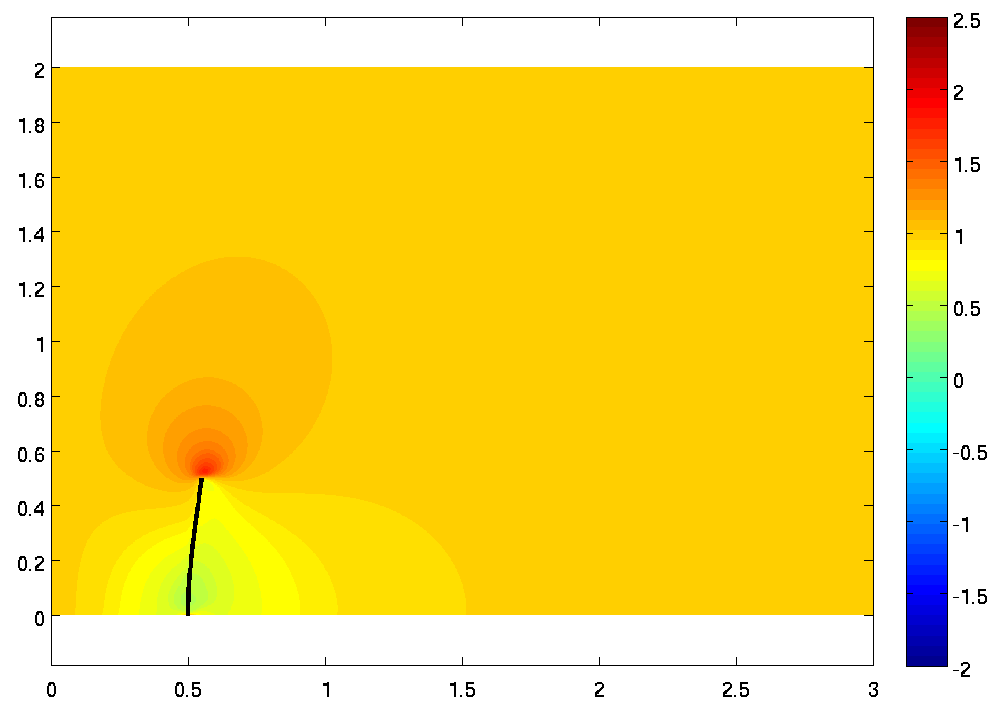
\includegraphics[width=4.25cm]{Chapter_5/figure/monofin_L05_t01_U.png}
    }
    \quad
    \subfigure[$t = 2.0 \text{ sec}$]
    {
    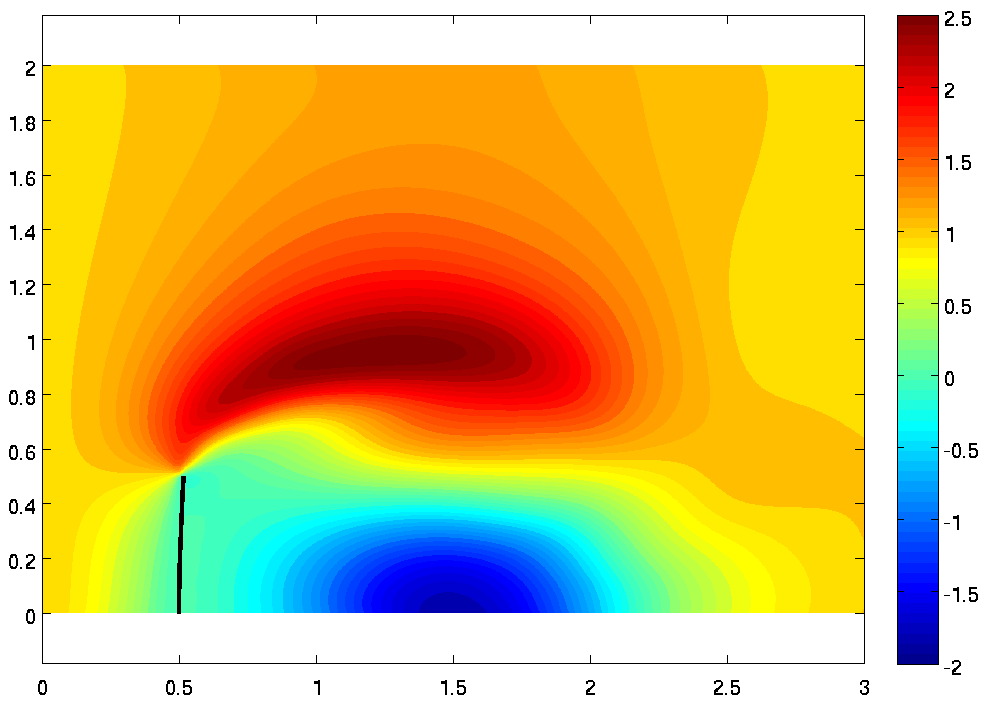
\includegraphics[width=4.25cm]{Chapter_5/figure/monofin_L05_t20_U.png}
    }
    \quad
    \subfigure[$t = 5.0 \text{ sec}$]
    {
    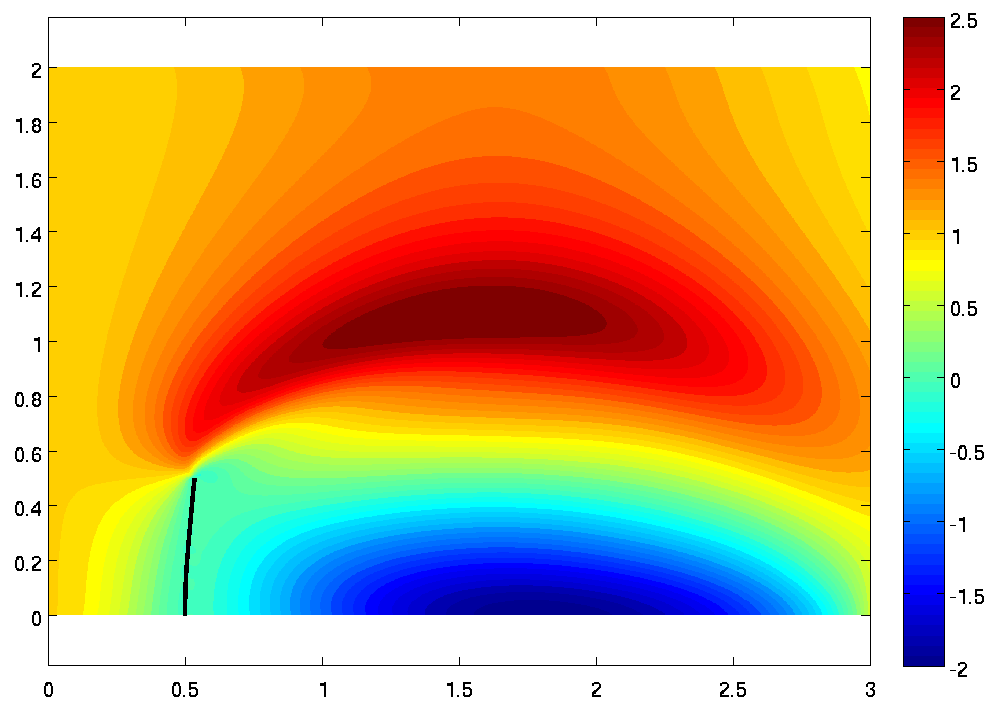
\includegraphics[width=4.25cm]{Chapter_5/figure/monofin_L05_t50_U.png}
    }
    \\
    \subfigure[$t = 0.1 \text{ sec}$]
    {
    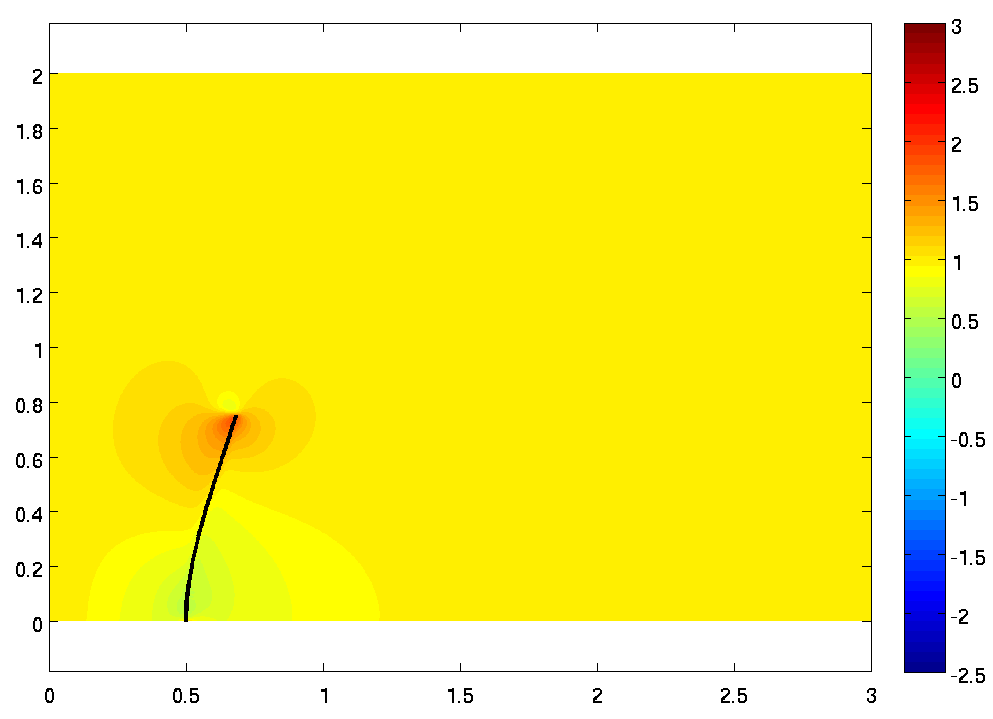
\includegraphics[width=4.25cm]{Chapter_5/figure/monofin_L75_t01_U.png}
    }
    \quad
    \subfigure[$t = 2.0 \text{ sec}$]
    {
    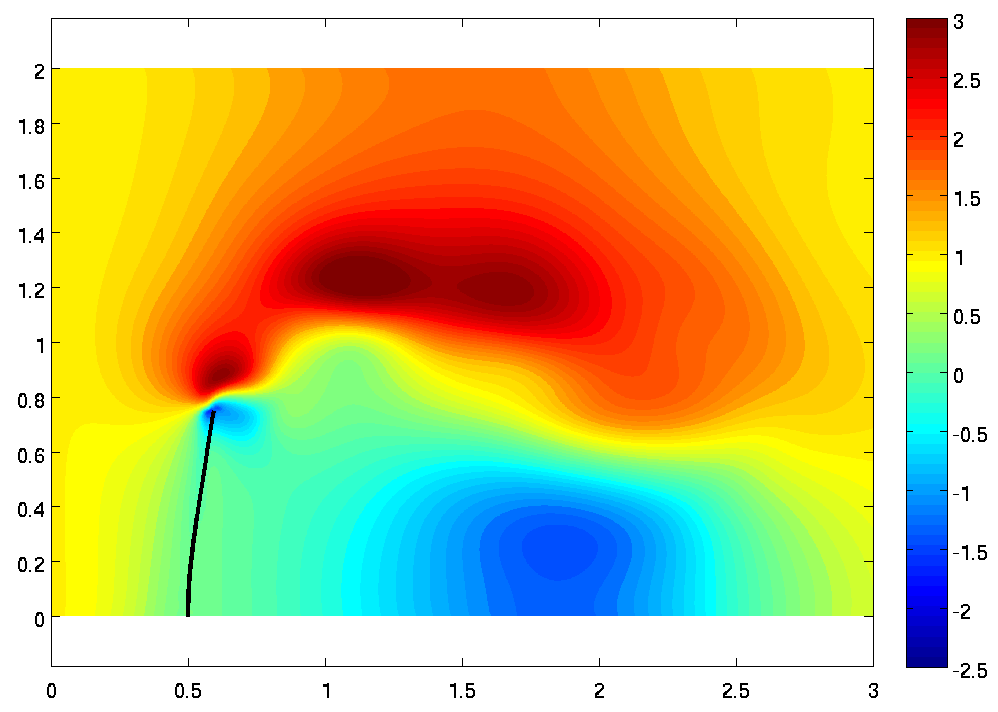
\includegraphics[width=4.25cm]{Chapter_5/figure/monofin_L75_t20_U.png}
    }
    \quad
    \subfigure[$t = 5.0 \text{ sec}$]
    {
    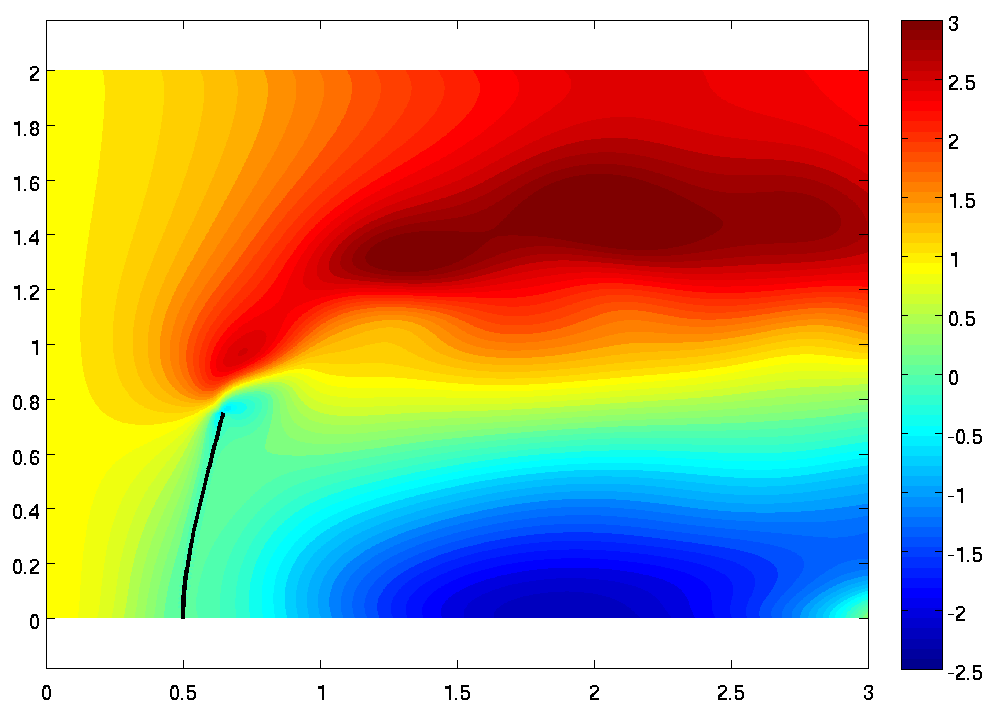
\includegraphics[width=4.25cm]{Chapter_5/figure/monofin_L75_t50_U.png}
    }
    \caption{U-velocity time snapshots for elastic monofin.}
    \label{fig:C5_monofinTimeSnapShotVelocity}
\end{figure}
%
%
\begin{figure}[H]
    \centering
    \subfigure[$t = 0.1 \text{ sec}$]
    {
    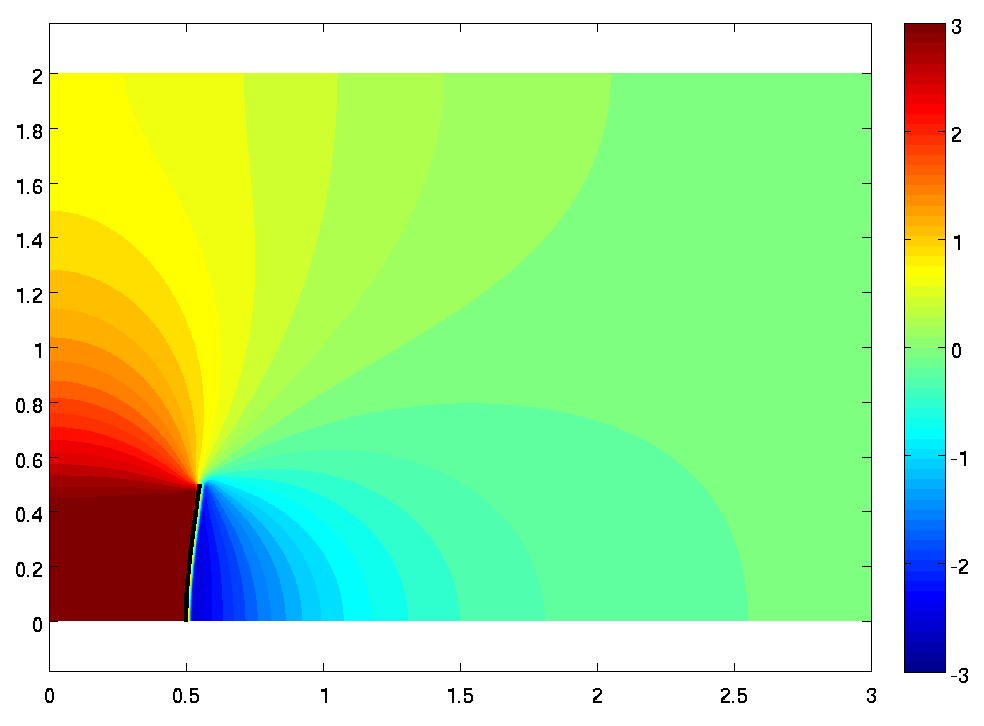
\includegraphics[width=4.25cm]{Chapter_5/figure/monofin_L05_t01_P.png}
    }
    \quad
    \subfigure[$t = 2.0 \text{ sec}$]
    {
    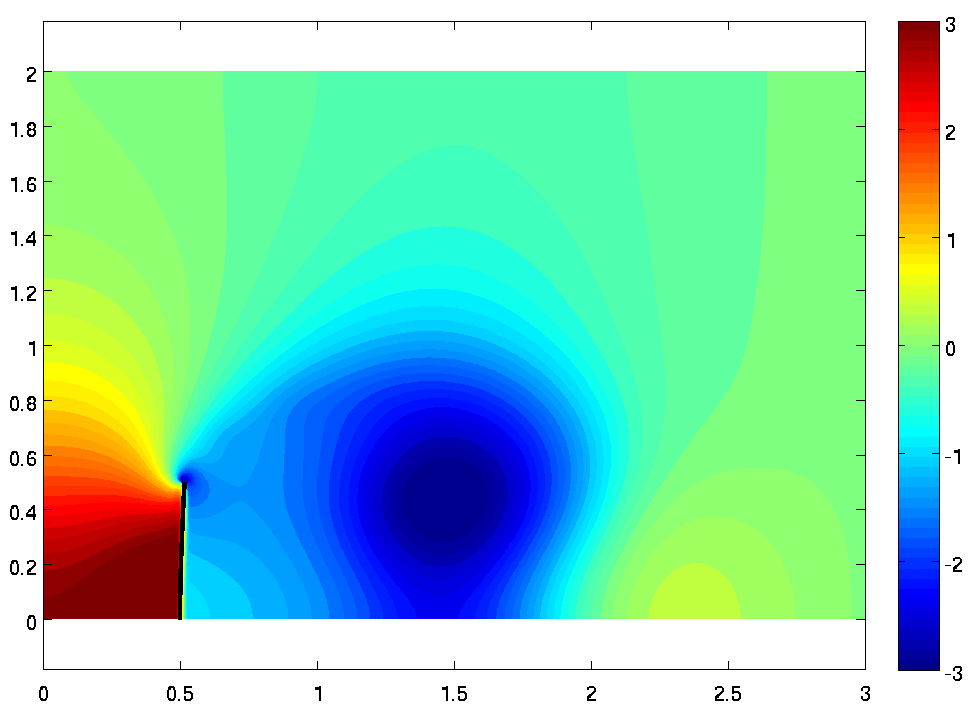
\includegraphics[width=4.25cm]{Chapter_5/figure/monofin_L05_t20_P.png}
    }
    \quad
    \subfigure[$t = 5.0 \text{ sec}$]
    {
    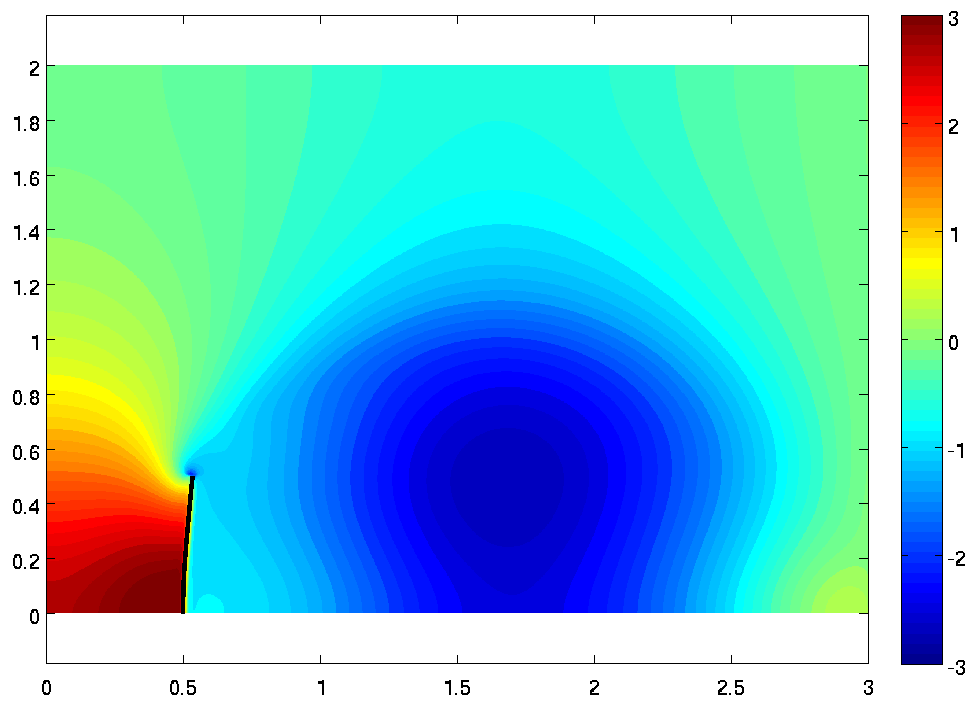
\includegraphics[width=4.25cm]{Chapter_5/figure/monofin_L05_t50_P.png}
    }
    \\
    \subfigure[$t = 0.1 \text{ sec}$]
    {
    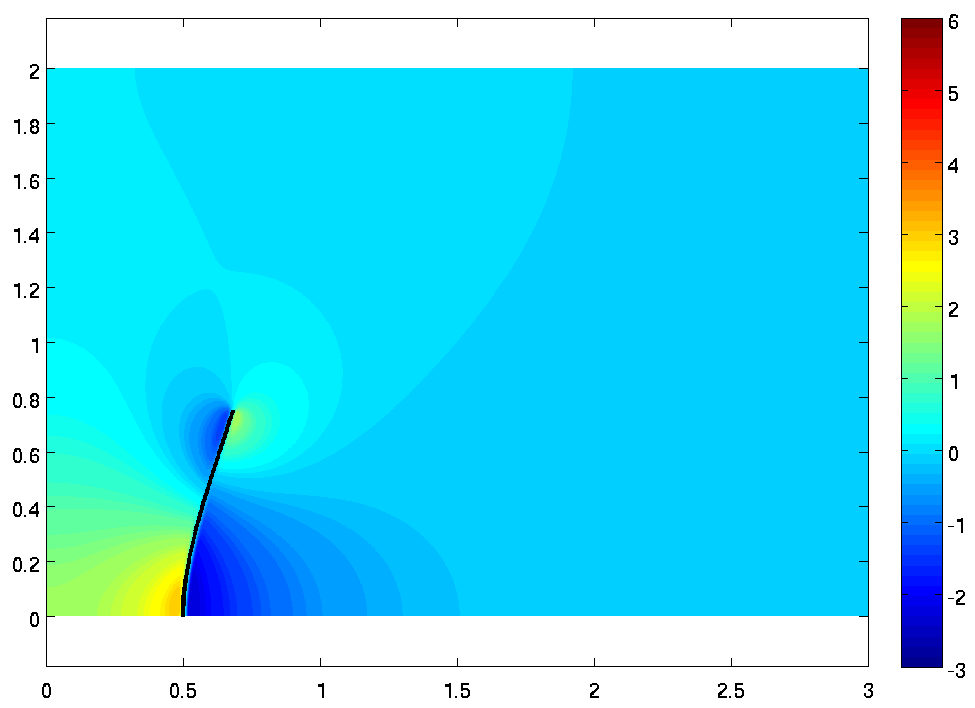
\includegraphics[width=4.25cm]{Chapter_5/figure/monofin_L75_t01_P.png}
    }
    \quad
    \subfigure[$t = 2.0 \text{ sec}$]
    {
    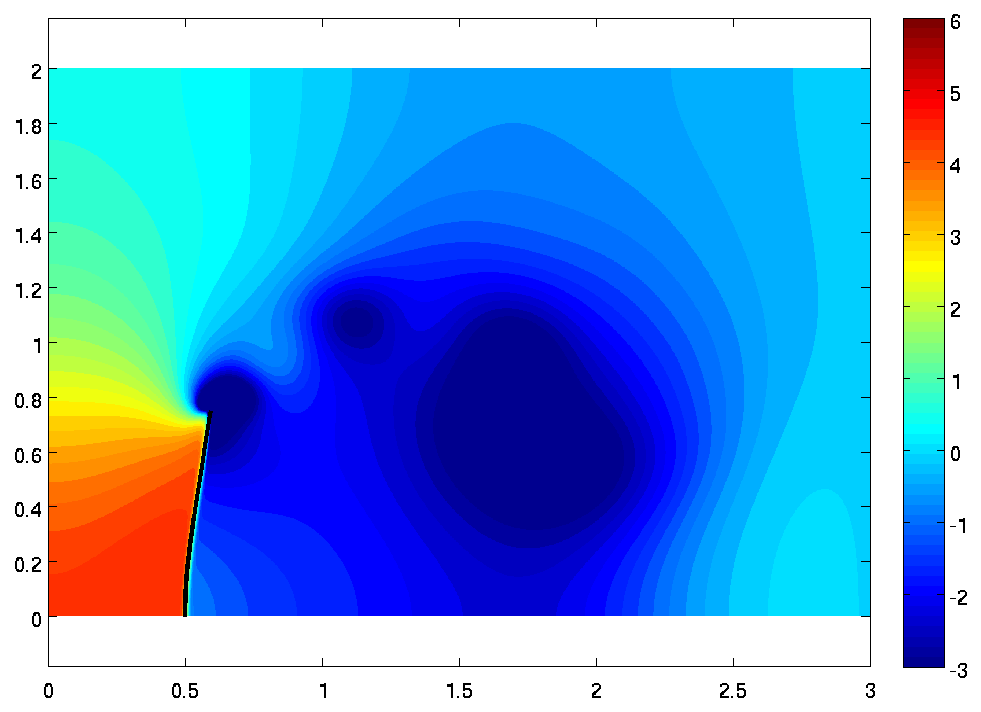
\includegraphics[width=4.25cm]{Chapter_5/figure/monofin_L75_t20_P.png}
    }
    \quad
    \subfigure[$t = 5.0 \text{ sec}$]
    {
    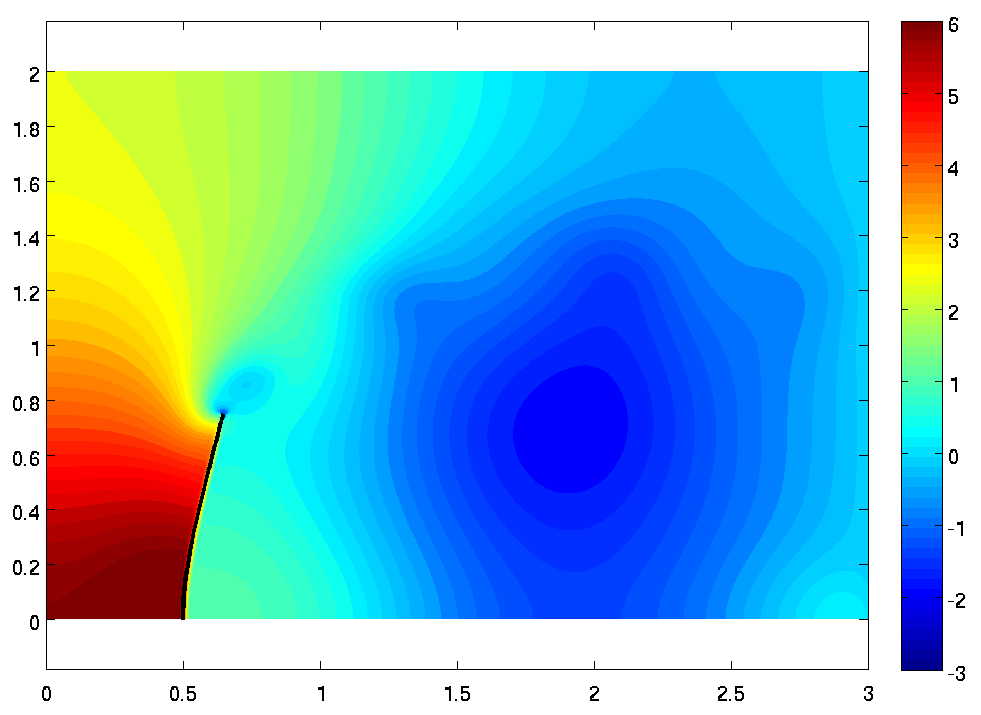
\includegraphics[width=4.25cm]{Chapter_5/figure/monofin_L75_t50_P.png}
    }
    \caption{Pressure time snapshots for elastic monofin.}
    \label{fig:C5_monofinTimeSnapShotPressure}
\end{figure}
%
We calculate the monofin tip displacement sensitivity to its length, that affects both the fluid and structure domain. Therefore, both of the governing equations need to be differentiated with respect to the length. Differentiation of the Navier-stokes equations for the fluid is extensively discussed in Chapter \ref{ch:shapeSenwithIB}, here we derive the continuum sensitivity equation for the monofin structure. The governing equation for an Euler-Bernoulli beam is shown in Equation \eqref{eq:C5_eulerBernoulliBeamGE}.
%
\begin{equation}\label{eq:C5_eulerBernoulliBeamGE}
	\frac{d^2}{dx^2}
	\left( EI \frac{d^2 w}{dx^2} \right) + \rho \frac{d^2 w}{dt^2} = q(x)
\end{equation}
%
where $w$ is the deflection in $y$ direction; $E$ is elastic modulus; $I$ is the second moment of area of the beam's cross-section; $\rho$ is mass per length; and $q(x)$ is the distributed load. The sensitivity equation for the structure is derived by analytically differentiating Equation \eqref{eq:C5_eulerBernoulliBeamGE} with respect to design variable $L$ as shown in Equation \eqref{eq:C5_eulerBernoulliBeamSE}.
%
\begin{equation}\label{eq:C5_eulerBernoulliBeamSE}
	\frac{d^2}{dx^2}
	\left( EI \frac{d^2 w'}{dx^2} \right) + \rho \frac{d^2 w'}{dt^2} = q'(x)
\end{equation}
%
where $( )'$ represents the derivative of response with respect to design variable, $L$. It should be noted that the right-hand side of Equations \eqref{eq:C5_eulerBernoulliBeamGE} and \eqref{eq:C5_eulerBernoulliBeamSE} are solved by solving the Navier-Stokes and differentiated Navier-Stokes equations, respectively. The loads from the fluid domain are transferred to the structure using regularized delta function. The time history of the sensitivity of tip displacement to the length of the monofin is shown in Figure \ref{fig:C5_timeHistoryTipDisplacementSensitivity}. As shown here, the sensitivity results from the CSA agrees well with the Complex Step (CS) results.
%
\begin{figure}[H]
    \centering
    \subfigure[$L = 0.5 \text{ m}$]
    {
    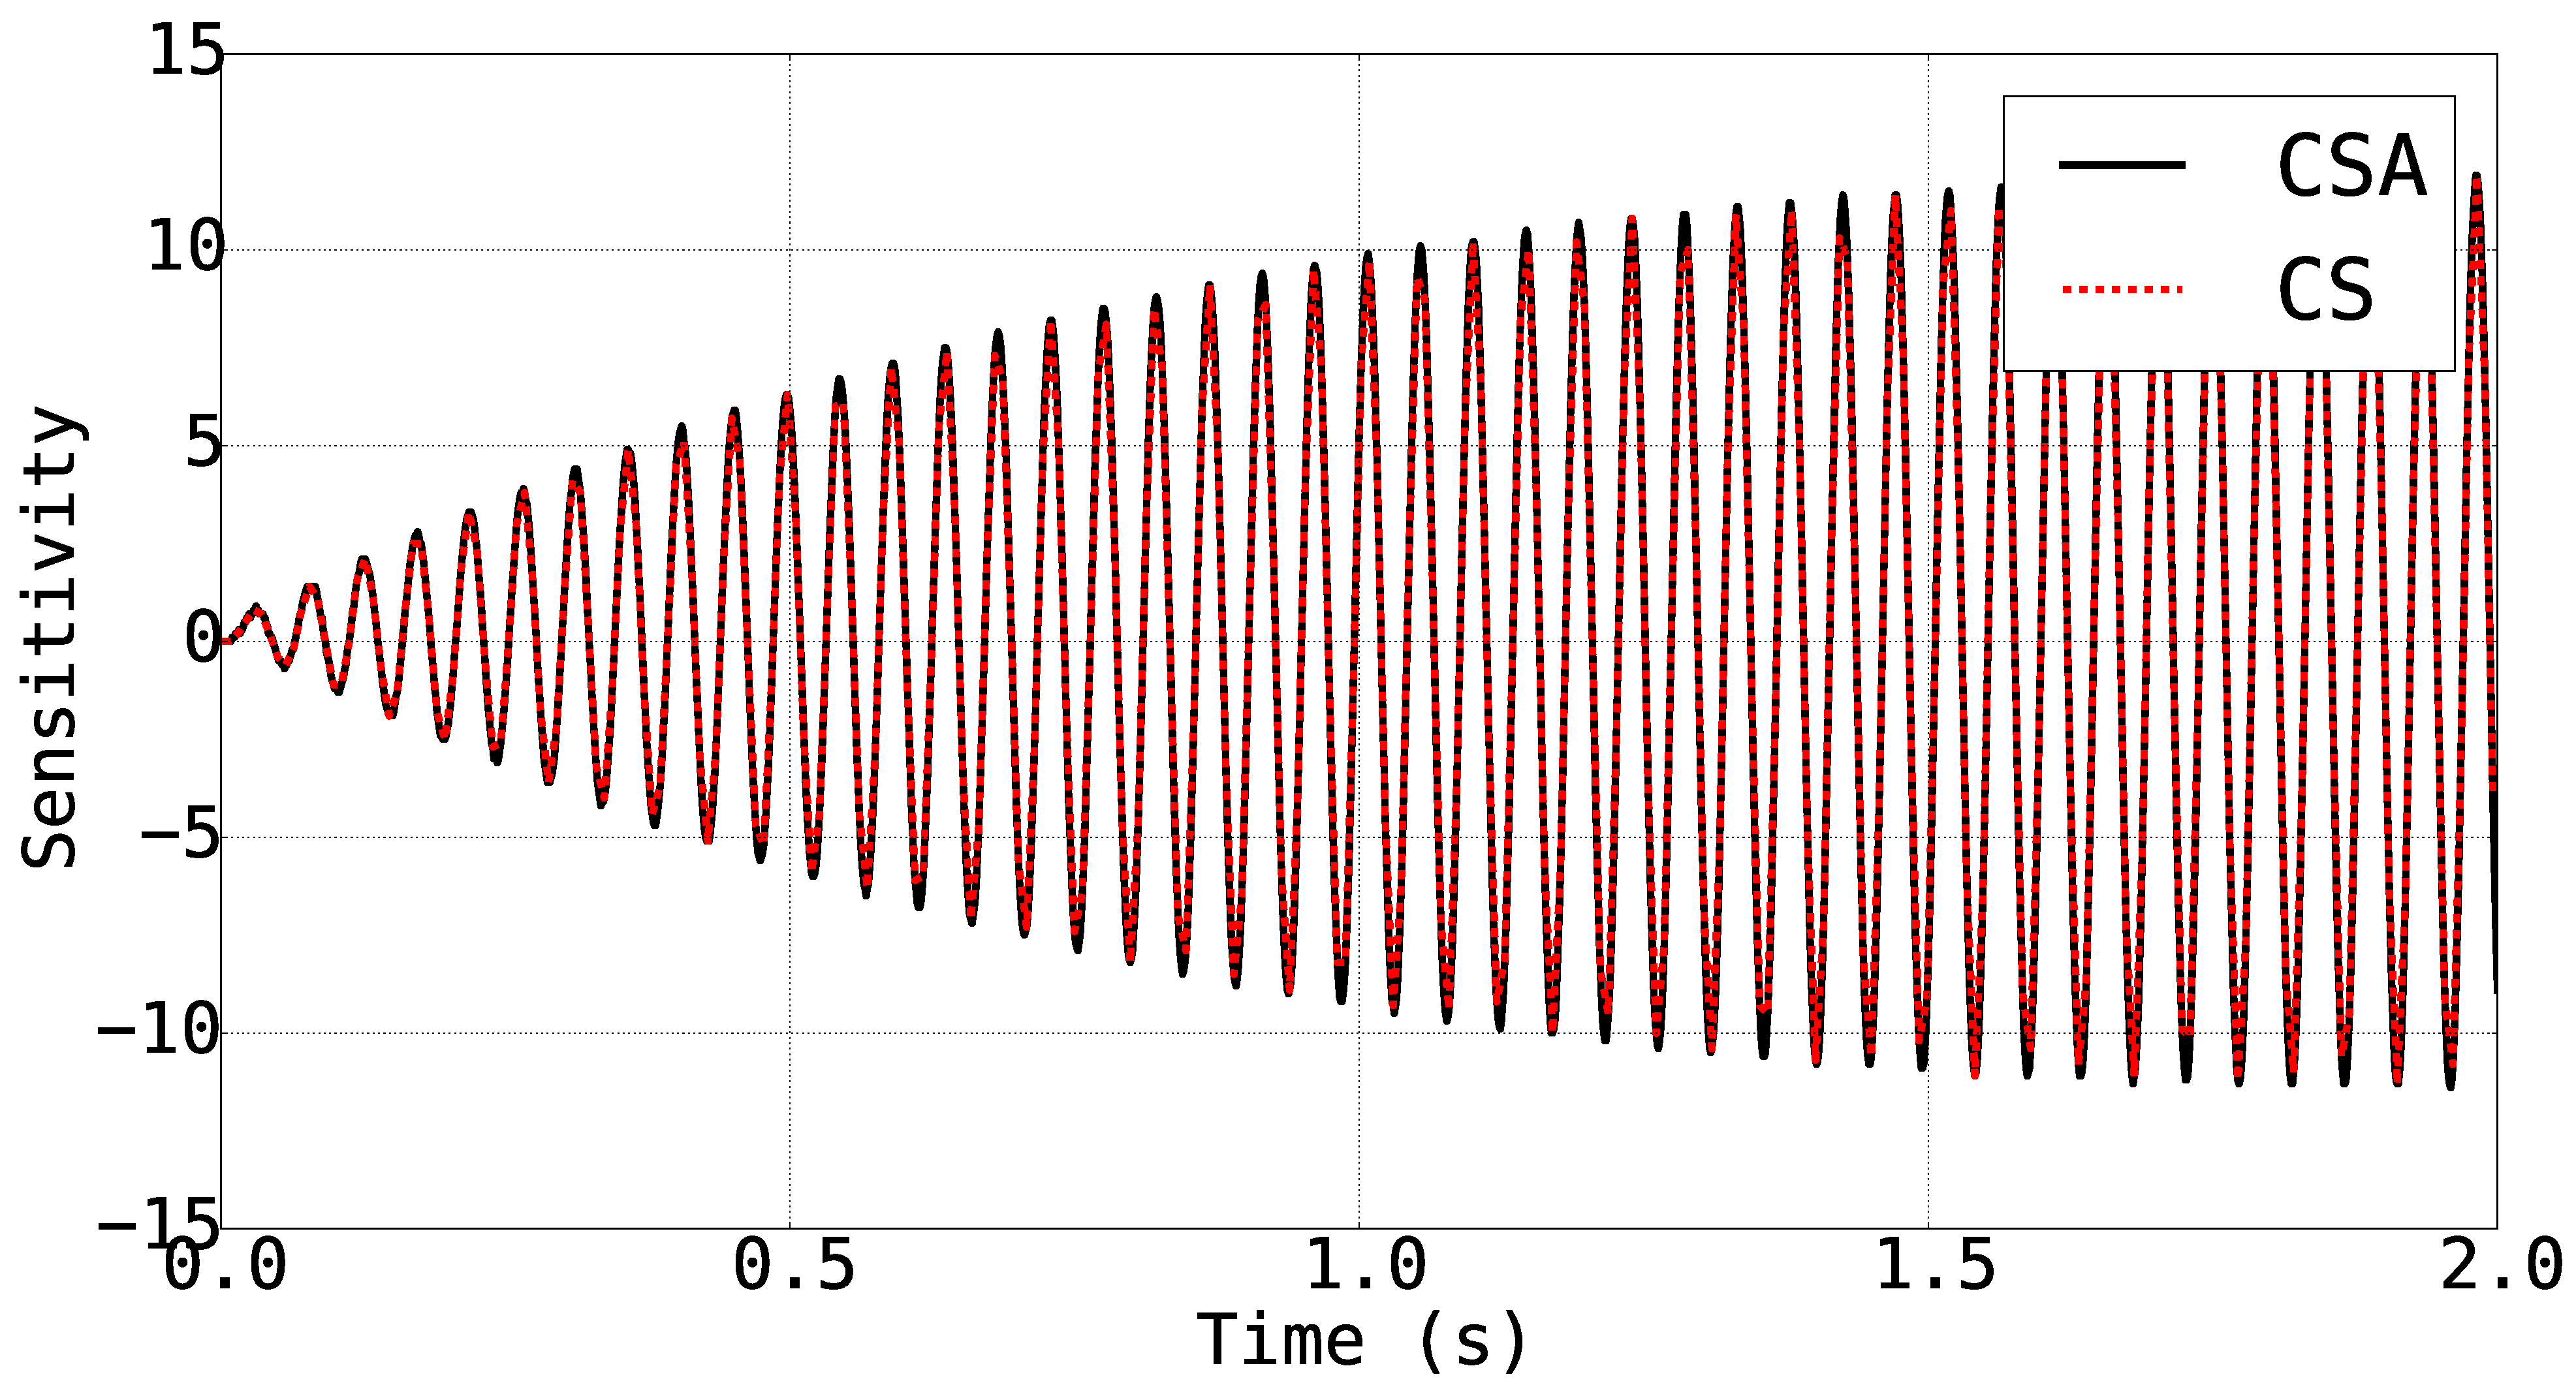
\includegraphics[width=6.5cm]{Chapter_5/figure/monofin_L05_dispSensitivity.eps}
    \label{fig:C5_thinAirfoil}
    }
    \quad
    \subfigure[$L = 0.75 \text{ m}$]
    {
    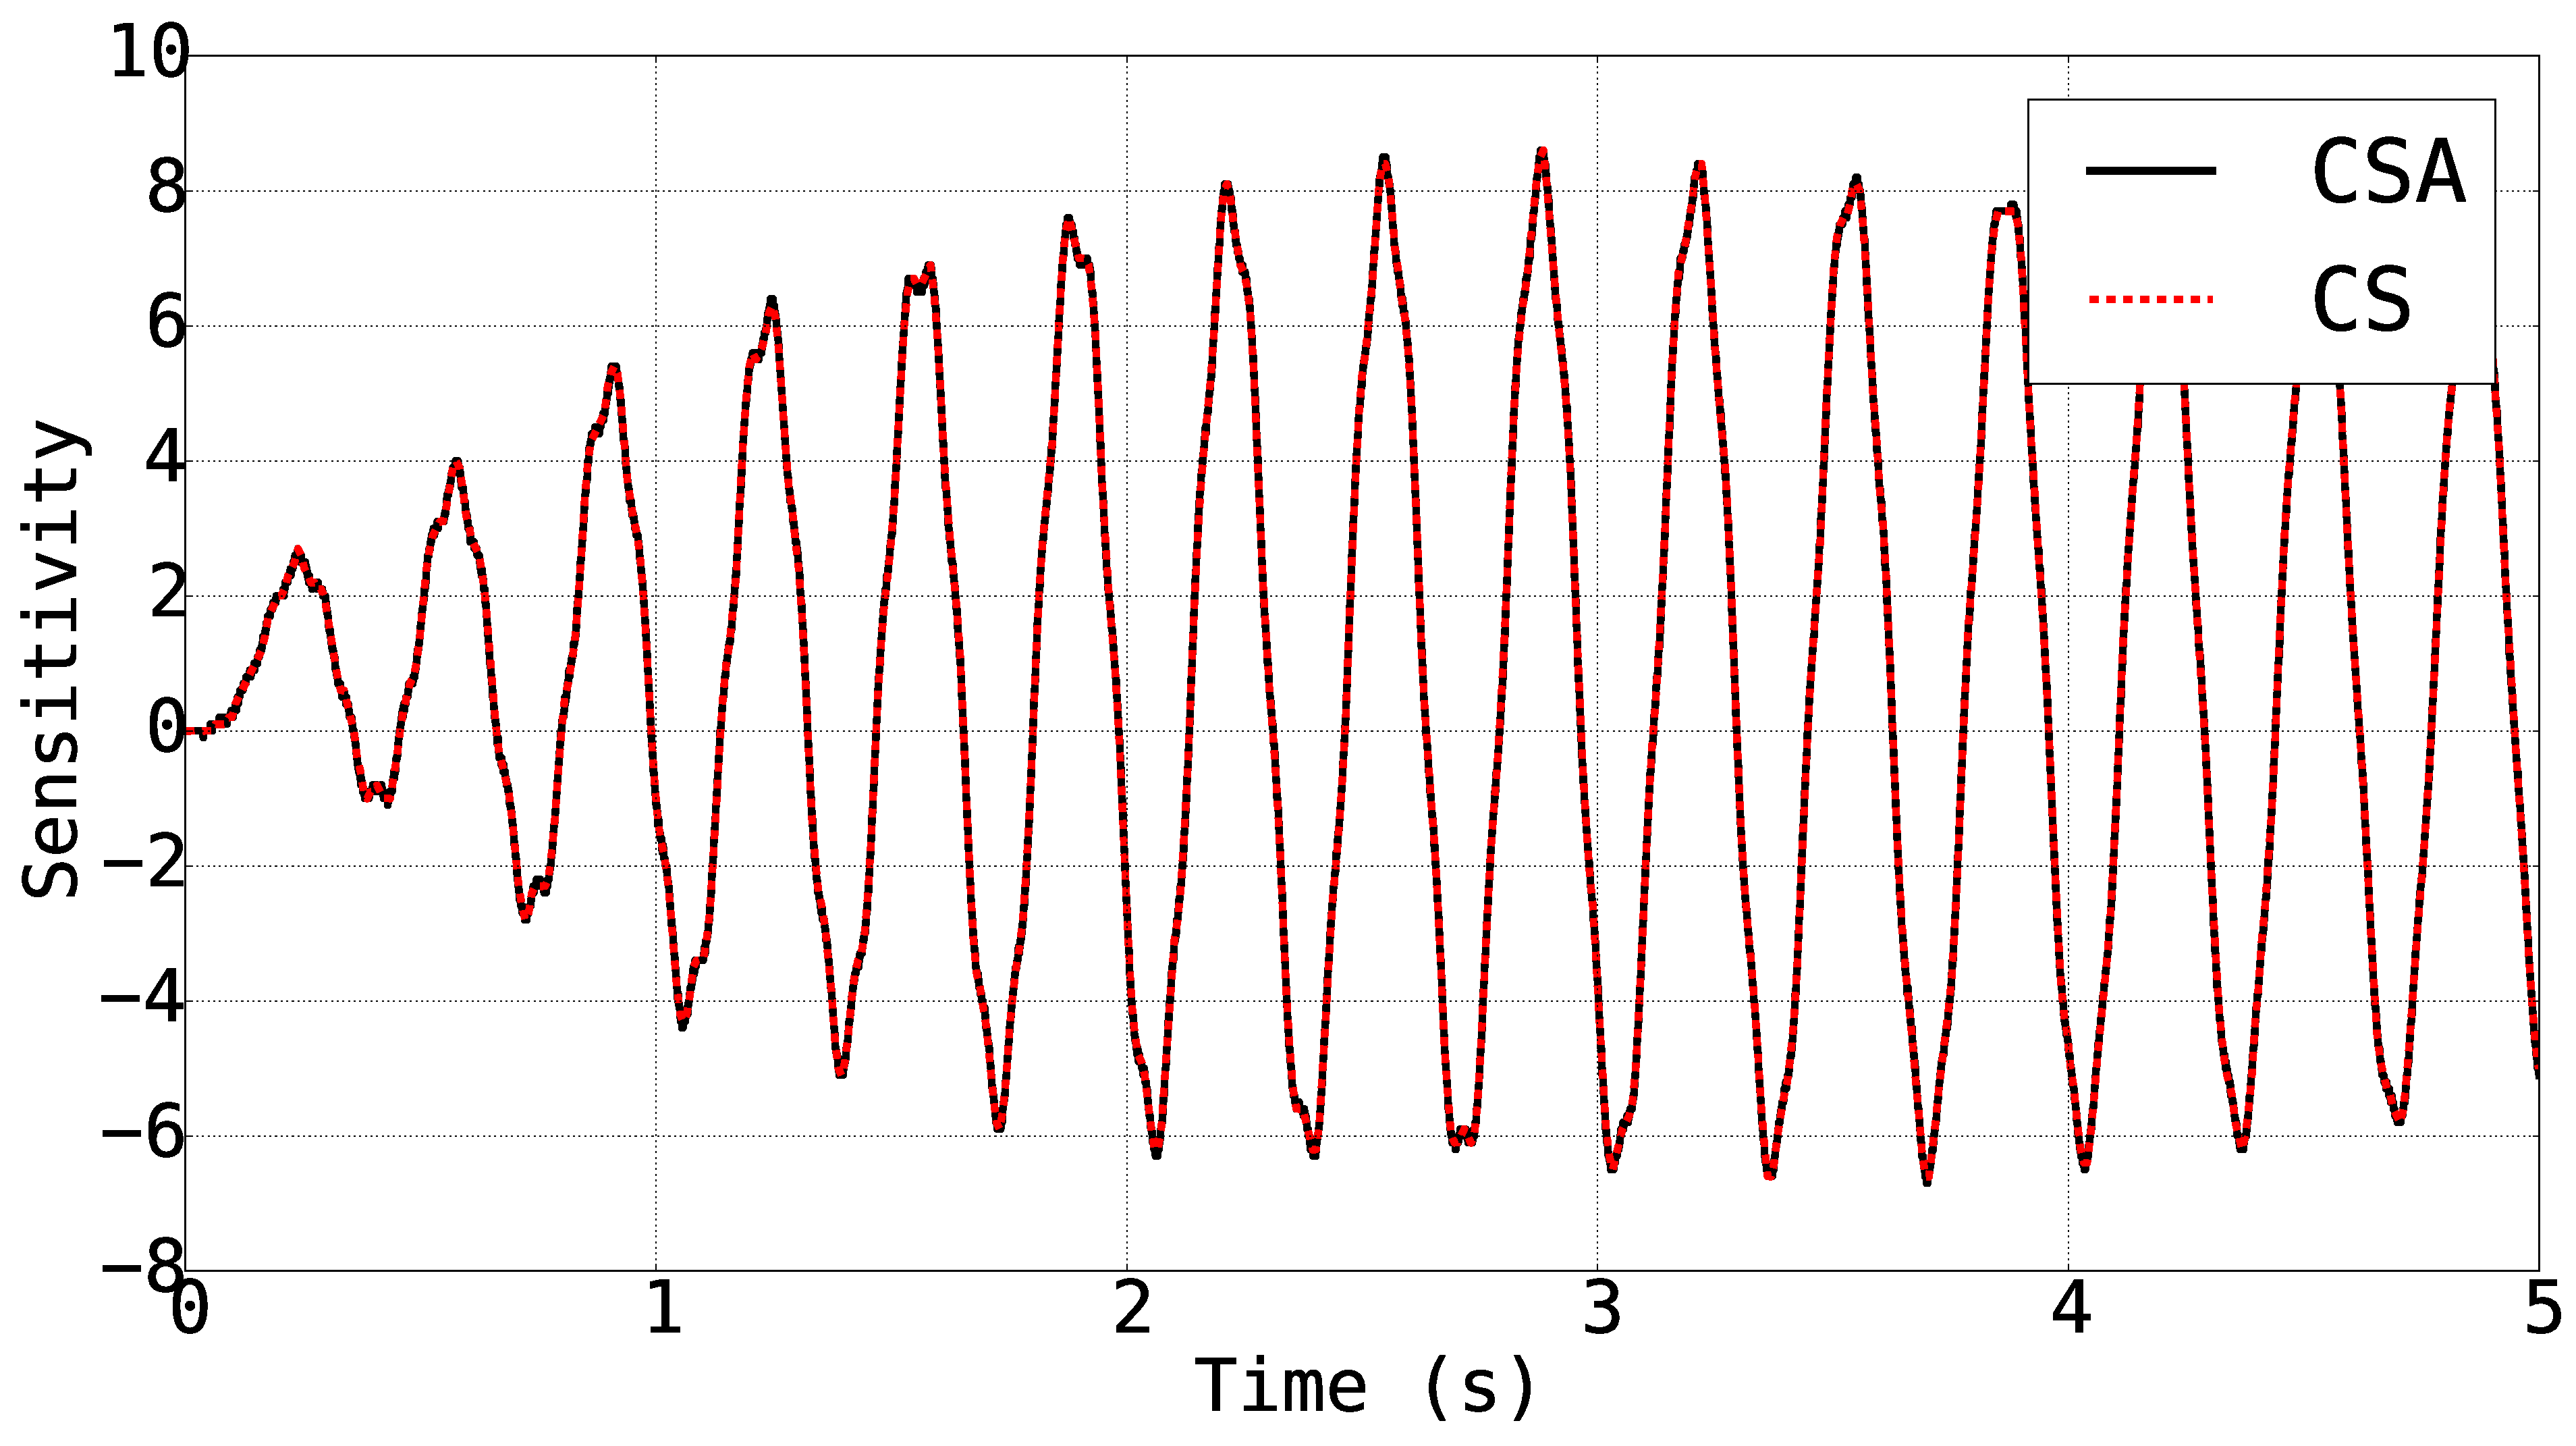
\includegraphics[width=6.5cm]{Chapter_5/figure/monofin_L75_dispSensitivity.eps}
    \label{fig:C5_thickAirfoil}
    }
    \caption{Time history of the monofin tip displacement in cross-flow.}
    \label{fig:C5_timeHistoryTipDisplacementSensitivity}
\end{figure}
%
